\documentclass{subfiles}

\begin{document}

    \chapter{Análisis y diseño}
    \label{chap:analisis_y_diseno}

        \section{Análisis de requisitos}
        \label{sec:analisis_de_requisitos}
        A continuación se enumerarán los requisitos del proyecto que se han obtenido a través de diferentes sesiones de estudio de diferentes productos similares en el mercado. A través de estos, se puede obtener una idea básica del producto a obtener.

        \subsection{Requisitos funcionales}
        \label{sec:requisitos_funcionales}

%%%%%%%%%%%%%%%%%%%%%%%%%
%% REQUISITOS FUNCIONALES
%%%%%%%%%%%%%%%%%%%%%%%%%
\begin{longtblr}[
  caption = {Requisitos funcionales del sistema},
  label = {tab:requisitos_funcionales_del_sistema},
]{
  width = \linewidth,
  colspec = {Q[100]Q[842]},
  column{1} = {c},
  hlines,
  vlines,
}
\textbf{Código} & \textbf{Descripción}\\
RF01 & El sistema será capaz de obtener imágenes de la cámara de un dispositivo móvil\\
RF02 & El sistema será capaz de cargar modelos tridimensionales\\
RF03 & El sistema será capaz de insertar renderizaciones de modelos tridimensionales sobre otras imágenes\\
RF04 & El sistema será capaz de detectar el movimiento del dispositivo utilizado\\
RF05 & El sistema será capaz de iniciar una sesión de \ra \\
RF06 & El sistema será capaz de reproducir pistas de audio con efecto espacial\\
RF07 & El sistema será capaz de animar modelos tridimensionales\\
RF08 & El sistema será capaz de detectar superficies en imágenes captadas por el dispositivo móvil\\
RF09 & El sistema será capaz de ubicar figuras tridimensionales en superficies encontradas en imágenes\\
RF10 & El sistema será capaz de modificar la ubicación de una figura tridimensional\\
RF11 & El sistema será capaz de modificar la ubicación de un sonido espacial\\
RF12 & El sistema será capaz de modificar la orientación de la figura tridimensional en relación al movimiento del dispositivo\\
RF13 & El sistema será capaz de obtener modelos tridimensionales de una URL dada\\
RF14 & El sistema será capaz de cargar un modelo aleatorio de entre varios dados\\
RF15 & El sistema será capaz de detener la animación al cerrarse la sesión de \ra \\
RF16 & El sistema será capaz de detener la pista de audio reproducida al cerrarse la sesión de \ra
\end{longtblr}

%%%%%%%%%%%%%%%%%%%%%%%%%%%%%
%% FIN REQUISITOS FUNCIONALES
%%%%%%%%%%%%%%%%%%%%%%%%%%%%%

        \subsection{Requisitos no funcionales}
        \label{sec:requisitos_no_funcionales}

%%%%%%%%%%%%%%%%%%%%%%%%%%%%
%% REQUISITOS NO FUNCIONALES
%%%%%%%%%%%%%%%%%%%%%%%%%%%%
\begin{longtblr}[
  caption = {Requisitos no funcionales del sistema},
  label = {tab:requisitos_no_funcionales_del_sistema},
]{
  width = \linewidth,
  colspec = {Q[100]Q[842]},
  column{1} = {c},
  hlines,
  vlines,
}
\textbf{Código} & \textbf{Descripción}\\
RNF01 & El sistema deberá poder utilizarse en dispositivos móviles\\
RNF02 & El sistema deberá poder utilizarse en el sistema operativo \android \\
RNF03 & El sistema deberá poder utilizarse en el navegador \googlechrome para \android \\
RNF04 & El sistema deberá estar alojado en un servidor \linux \\
RNF05 & El sistema deberá ser accesible a través de un código QR\\
RNF06 & El sistema deberá cargar la \textit{landing page} en menos de 2 segundos\\
RNF07 & El sistema deberá cargar el modelo tridimensional en menos de 5 segundos
\end{longtblr}

%%%%%%%%%%%%%%%%%%%%%%%%%%%%%%%%
%% FIN REQUISITOS NO FUNCIONALES
%%%%%%%%%%%%%%%%%%%%%%%%%%%%%%%%

        \section{Casos de uso}
        \label{sec:casos_de_uso}

        \section{Modelo de dominio}
        \label{sec:modelo_de_dominio}

        \section{Diagramas}
        \label{sec:diagramas}

        \section{Estructura}
        \label{sec:estructura}
        Debido a la clara repartición de tareas en cada sección del código, se ha pretendido aplicar una separación tipo Modelo-Vista-Controlador en la aplicación, de manera que todo esté visiblemente separado y se pueda utilizar un sistema de orientación a objetos en toda la parte escrita en \js.

        \paragraph{}
        La primera sección a comentar sería el Modelo. En esta aplicación, tal y como se ha planteado el desarrollo y teniendo en cuenta qué librerías externas se han incorporado y cómo se han utilizado, se ha tratado a estas como si fueran el propio Modelo. Así, nuestra información es en sí las librerías externas añadidas, que serán además las que se encarguen de cargar los datos estáticos de servidor: los modelos en 3D y las grabaciones de las voces de estos.

        \paragraph{}
        La segunda sección sería la Vista. En este caso, la Vista de esta aplicación constaría únicamente de un HTML llamado \textit{index}, que sería además la \textit{landing page} de la aplicación. Sobre esta misma página será sobre la que se colocará más tarde un \textit{<<canvas>>}, que es el elemento HTML que permite mostrar elementos gráficos de manera dinámica a través de \js. Utilizando este último podremos mostrar las imágenes captadas a través de la cámara del dispositivo móvil y mezclarlas con los modelos en 3D para generar nuestra \ra.

        \paragraph{}
        Por último, la sección restante sería el Controlador. En este, se procesan todos los eventos generados por el usuario, además de tratar toda la información que se recibirá de los sensores del dispositivo para poder generar las imágenes de manera verosímil. En este se ubicará un bucle que se ocupará de obtener la imagen a mostrar, mezclarla con el modelo en 3D, renderizar la imagen y situarla en la vista, todo esto de la manera más fluida posible para que el espectador no tenga impresiones que entorpezcan la experiencia de usuario.

        \paragraph{}
        Además, esta almacenará también información de la Sesión necesaria para el correcto procesamiento del sistema, tales como los modelos en 3D cargados, la referencia al objeto de \js con el \textit{<<canvas>>} antes mencionado, la posición del usuario y otros datos necesarios para el funcionamiento del sistema que serán mencionados a lo largo de esta memoria.

        \paragraph{}
        Es importante mencionar que, a pesar de que se ha tratado a este sistema como un Modelo-Vista-Controlador y se le ha presentado como tal, sería más justo tratar a la aplicación como si utilizara el patrón Modelo-Vista-Presentador \cite{web:mvp} por varias razones.

        \paragraph{}
        La primera es que no tenemos constancia de cómo almacenan estas librerías las pocas referencias que se le entregan a la Vista y, aún manteniendo esta referencia como si lo tratara como la Vista en este tipo de patrones, no parece realizar cambios sobre esta de manera directa.

        \paragraph{}
        La segunda es que las actualizaciones se realizan directamente desde el Controlador, siendo necesario realizar desde este último acciones explícitas para actualizar la apariencia de la vista, como por ejemplo el renderizado de la imagen a mostrar en pantalla.

        \paragraph{}
        Por último y más importante, es necesario que todos los cambios estén revisados en el bucle que se genera en el Controlador, el cual se tratará más adelante. Esto obliga a este último a solicitar información continuamente a las librerías, hacer cálculos y mostrarlos en pantalla, mientras está atento a los eventos de los usuarios.

        \begin{figure}
        \centering
        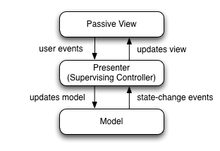
\includegraphics[width=0.5\textwidth]{img/mvp.png}
        \caption{Representación gráfica del patrón Modelo-Vista-Presentador. Fuente: \citetitle{web:wikipedia_modelviewpresenter}.}
        \label{fig:mvp}
        \end{figure}

        \paragraph{}
        Por todo esto, y dado que la lógica de negocio está separada de la interfaz de usuario, la estructura se corresponde con el patrón Modelo-Vista-Presentador. Sin embargo, dado que desde el inicio del proyecto se trató cada parte como el clásico Modelo-Vista-Controlador, y dado que el Modelo-Vista-Presentador proviene de este último, cada parte será nombrada como si lo fuera, aún siendo conscientes de las diferencias.

        \section{Capas}
        \label{sec:capas}

        \section{Arquitectura y diseño de datos}
        \label{sec:arquitectura_y_diseno_de_datos}

\end{document}